\documentclass[10pt,onecolumn,letterpaper]{article}

\usepackage{iccv}
\usepackage{times}
\usepackage{epsfig}
\usepackage{graphicx}
\usepackage{amsmath}
\usepackage{amssymb}
\usepackage[square,numbers,sort&compress]{natbib}

\usepackage{subfigure}
\usepackage{upgreek}
\usepackage{multirow}
\usepackage{color}
\usepackage{bm}
\DeclareMathOperator*{\argmin}{arg\,min}
\usepackage{arydshln}
\usepackage{latexsym}

\usepackage{amsthm}
\newtheorem{theorem}{Theorem}
\newtheorem{lemma}[theorem]{Lemma}
\newtheorem{conj}[theorem]{Conjecture}


\usepackage{authblk}
\usepackage{xpatch}
\setlength{\bibsep}{0.4ex}  % vertical spacing between references

\usepackage{lipsum}
% ADD THE FOLLOWING COUPLE LINES INTO YOUR PREAMBLE
\let\OLDthebibliography\thebibliography
\renewcommand\thebibliography[1]{
  \OLDthebibliography{#1}
  \setlength{\parskip}{0pt}
  \setlength{\itemsep}{0.2pt plus 0.05ex}
}

% Include other packages here, before hyperref.

% If you comment hyperref and then uncomment it, you should delete
% egpaper.aux before re-running latex.  (Or just hit 'q' on the first latex
% run, let it finish, and you should be clear).
\usepackage[pagebackref=true,breaklinks=true,letterpaper=true,colorlinks,bookmarks=false]{hyperref}
\renewcommand{\huge}{\fontsize{8.775pt}{\baselineskip}\selectfont}
\renewcommand{\Huge}{\fontsize{8pt}{\baselineskip}\selectfont}

% Include other packages here, before hyperref.

% If you comment hyperref and then uncomment it, you should delete
% egpaper.aux before re-running latex.  (Or just hit 'q' on the first latex
% run, let it finish, and you should be clear).
\usepackage[breaklinks=true,bookmarks=false]{hyperref}

\iccvfinalcopy % *** Uncomment this line for the final submission

\def\iccvPaperID{****} % *** Enter the ICCV Paper ID here
\def\httilde{\mbox{\tt\raisebox{-.5ex}{\symbol{572}}}}

% Pages are numbered in submission mode, and unnumbered in camera-ready
%\ificcvfinal\pagestyle{empty}\fi
% \setcounter{page}{}


\begin{document} 

%%%%%%%%% TITLE
\title{Supplementary Materials to ``Multi-channel Weighted Nuclear Norm Minimization for Real Color Image Denoising''}
\vspace{-4mm}
\xpatchcmd{\author}{\relax#1\relax}{\relax\detokenize{#1}\relax}{}{}
\author[1]{Jun Xu}
\author[\empty]{Lei Zhang\textsuperscript{1,}\thanks{This work is supported by HK RGC GRF grant (PolyU 5313/13E) and China NSFC grant (no. 61672446).}}
\author[1]{David Zhang}
\author[2]{Xiangchu Feng}
\affil[1]{Dept. of Computing, The Hong Kong Polytechnic University, Hong Kong, China}
\affil[2]{School of Mathematics and Statistics, Xidian University, Xi'an, China 
\authorcr{\tt \small{\{csjunxu,cslzhang,csdzhang\}@comp.polyu.edu.hk,xcfeng@mail.xidian.edu.cn}}
}
\vspace{-4mm}

\maketitle
\vspace{-4mm}
%\thispagestyle{empty}


In this supplementary file, we provide:\vspace{-2mm}
\begin{enumerate}
\item The proof of the Theorem 1 in the main paper;
\vspace{-2mm}
\item More denoising results on the Kodak PhotoCD dataset;
\vspace{-2mm}
\item More visual comparisons of denoised images on the real noisy images of dataset \cite{ncwebsite}; 
\vspace{-2mm}
\item More visual comparisons of denoised images on the real noisy images of dataset \cite{crosschannel2016}.
\end{enumerate}

\section{Proof of Theorem 1.}
\begin{theorem}
Assume that the weights in $\bm{w}$ are in a non-descending order, the sequence $\{\bm{X}_{k}\}$, $\{\bm{Z}_{k}\}$, and $\{\bm{A}_{k}\}$ generated in Algorithm 1 satisfy:
\begin{equation}
(a) \lim_{k \to \infty} \|\bm{X}_{k+1}-\bm{Z}_{k+1}\|_{F}=0;
\quad
(b) \lim_{k \to \infty} \|\bm{X}_{k+1}-\bm{X}_{k}\|_{F}=0;
\quad
(c) \lim_{k \to \infty} \|\bm{Z}_{k+1}-\bm{Z}_{k}\|_{F}=0.
\end{equation}
\end{theorem}
\begin{proof}
1.\ Firstly, we prove that the sequence $\{\bm{A}_{k}\}$ generated by Algorithm 1 is upper bounded.
Let $\bm{X}_{k+1}+\rho_{k}^{-1}\bm{A}_{k}
=
\bm{U}_{k}\bm{\Sigma}_{k}\bm{V}_{k}^{\top}$
be its singular value decomposition (SVD) \cite{eckart1936approximation} in the $(k+1)$-th iteration. According to Corollary 1 of \cite{wnnmijcv}, we can have the SVD of $\bm{Z}_{k+1}$ as $\bm{Z}_{k+1}=\bm{U}_{k}\hat{\bm{\Sigma}}_{k}\bm{V}_{k}^{\top}=\bm{U}_{k}\mathcal{S}_{\frac{\bm{w}}{\rho_{k}}}(\bm{\Sigma}_{k})\bm{V}_{k}^{\top}$. 
Then we have 
\begin{align}
\|
\bm{A}_{k+1}
\|_{F}
&
=
\|
\bm{A}_{k}
+
\rho_{k}
(\bm{X}_{k+1}-\bm{Z}_{k+1})
\|_{F}
=
\rho_{k}\|
\rho_{k}^{-1}
\bm{A}_{k}
+
\bm{X}_{k+1}
-
\bm{Z}_{k+1}
\|_{F}
\\
&
=
\rho_{k}\|
\bm{U}_{k}\bm{\Sigma}_{k}\bm{V}_{k}^{\top}
-
\bm{U}_{k}\mathcal{S}_{\frac{\bm{w}}{\rho_{k}}}(\bm{\Sigma}_{k})\bm{V}_{k}^{\top}
\|_{F}
=
\rho_{k}\|
\bm{\Sigma}_{k}
-
\mathcal{S}_{\frac{\bm{w}}{\rho_{k}}}(\bm{\Sigma}_{k})
\|_{F}
\\
&
=
\rho_{k}
\sqrt{\sum_{i}(\bm{\Sigma}_{k}^{ii}-\mathcal{S}_{\frac{w_{i}}{\rho_{k}}}(\bm{\Sigma}_{k}^{ii}))^{2}}
\le
\rho_{k}
\sqrt{\sum_{i}(\frac{w_{i}}{\rho_{k}})^{2}}
=
\sqrt{\sum_{i}w_{i}^{2}}.
\end{align}
The inequality in the second last step can be proved as follows: given the diagonal matrix $\bm{\Sigma}_{k}$, we define $\bm{\Sigma}_{k}^{ii}$ as the $i$-th element of $\bm{\Sigma}_{k}$. If $\bm{\Sigma}_{k}^{ii}\ge\frac{w_{i}}{\rho_{k}}$, we have $\mathcal{S}_{\frac{w_{i}}{\rho_{k}}}(\bm{\Sigma}_{k}^{ii})=\bm{\Sigma}_{k}^{ii}-\frac{w_{i}}{\rho_{k}}$. If $\bm{\Sigma}_{k}^{ii}<\frac{w_{i}}{\rho_{k}}$, we have $\mathcal{S}_{\frac{w_{i}}{\rho_{k}}}(\bm{\Sigma}_{k}^{ii})=0$. Overall, we have $|\bm{\Sigma}_{k}^{ii}-\mathcal{S}_{\frac{w_{i}}{\rho_{k}}}(\bm{\Sigma}_{k}^{ii})|\le\frac{w_{i}}{\rho_{k}}$ and hence the inequality holds. Hence, the sequence $\{\bm{A}_{k}\}$ is upper bounded.

2.\ Secondly, we prove that the sequence of Lagrangian function $\{\mathcal{L}(\bm{X}_{k+1},\bm{Z}_{k+1},\bm{A}_{k},\rho_{k})\}$ is also upper bounded. Since we have the globally optimal solution of $\bm{X}$ and $\bm{Z}$ in their corresponding subproblems, we always have 
\begin{align}
\mathcal{L}(\bm{X}_{k+1},\bm{Z}_{k+1},\bm{A}_{k},\rho_{k})
\le
\mathcal{L}(\bm{X}_{k},\bm{Z}_{k},\bm{A}_{k},\rho_{k}).
\end{align}
Based on the updating rule that 
$
\bm{A}_{k+1}
=
\bm{A}_{k} + \rho_{k}(\bm{X}_{k+1}-\bm{Z}_{k+1})
$
,
we have 
\begin{align}
&
\mathcal{L}(\bm{X}_{k+1},\bm{Z}_{k+1},\bm{A}_{k+1},\rho_{k+1})
\\
=
&
\mathcal{L}(\bm{X}_{k+1},\bm{Z}_{k+1},\bm{A}_{k},\rho_{k})
+
\langle
\bm{A}_{k+1}
-
\bm{A}_{k}
,
\bm{X}_{k+1}
-
\bm{Z}_{k+1}
\rangle
+
\frac{\rho_{k+1}-\rho_{k}}{2}
\|
\bm{X}_{k+1}-\bm{Z}_{k+1}
\|_{F}^{2}
\\
=
&
\mathcal{L}(\bm{X}_{k+1},\bm{Z}_{k+1},\bm{A}_{k},\rho_{k})
+
\frac{\rho_{k+1}+\rho_{k}}{2\rho_{k}^{2}}
\|
\bm{A}_{k+1}
-
\bm{A}_{k}
\|_{F}^{2}.
\end{align}
Since the sequence 
$\{
\bm{A}_{k}\}$
is upper bounded, the sequence 
$\{
\bm{A}_{k+1}
-
\bm{A}_{k}
\}$ is also upper bounded. Denote by $a$ the upper bound of 
$\{
\bm{A}_{k+1}
-
\bm{A}_{k}
\}$, 
i.e., 
$
\|
\bm{A}_{k+1}
-
\bm{A}_{k}
\|_{F}\le a
$
holds for
$\forall k\ge0$
,
we have 
\begin{align}
\mathcal{L}(\bm{X}_{k+1},\bm{Z}_{k+1},\bm{A}_{k+1},\rho_{k+1})
&
\le
\mathcal{L}(\bm{X}_{1},\bm{Z}_{1},\bm{A}_{0},\rho_{0})
+
a^2\sum_{k=0}^{\infty}\frac{\rho_{k+1}+\rho_{k}}{2\rho_{k}^{2}}
\\
&
=
\mathcal{L}(\bm{X}_{1},\bm{Z}_{1},\bm{A}_{0},\rho_{0})
+
a^2\sum_{k=0}^{\infty}\frac{\mu+1}{2\mu^{k}\rho_{0}}
\\
&
\le
\mathcal{L}(\bm{X}_{1},\bm{Z}_{1},\bm{A}_{0},\rho_{0})
+
\frac{a^2}{\rho_{0}}\sum_{k=0}^{\infty}\frac{1}{\mu^{k-1}}.
\end{align}
The last inequality holds since $\mu>1$ and $\mu+1<2\mu$. Therefore, we have $\sum_{k=0}^{\infty}\frac{1}{\mu^{k-1}}<\infty$ and the sequence of Lagrangian function 
$\{\mathcal{L}(\bm{X}_{k+1},\bm{Z}_{k+1},\bm{A}_{k+1},\rho_{k+1})\}$
is upper bounded.

3. Thirdly, we prove that the sequences of 
$\{\bm{X}_{k}\}$ and $\{\bm{Z}_{k}\}$ are upper bounded. Since 
\begin{align}
\|\bm{W}(\bm{Y}-\bm{X}_{k})\|_{F}^{2}
+
\|\bm{Z}_{k}\|_{\bm{w},*}
&
=
\mathcal{L}(\bm{X}_{k},\bm{Z}_{k},\bm{A}_{k-1},\rho_{k-1})
-
\langle
\bm{A}_{k-1},
\bm{X}_{k}-\bm{Z}_{k}
\rangle
-
\frac{\rho_{k-1}}{2}
\|
\bm{X}_{k}-\bm{Z}_{k}
\|_{F}^{2}
\\
&
=
\mathcal{L}(\bm{X}_{k},\bm{Z}_{k},\bm{A}_{k-1},\rho_{k-1})
+
\frac{1}{2\rho_{k-1}}
(
\|
\bm{A}_{k-1}
\|_{F}^{2}
-
\|
\bm{A}_{k}
\|_{F}^{2}
)
,
\end{align}
both $\{\bm{W}(\bm{Y}-\bm{X}_{k})\}$ and $\{\bm{Z}_{k}\}$ are upper bounded, and hence
the sequence $\{\bm{X}_{k}\}$ is bounded by the Cauchy-Schwarz inequality and triangle inequality.
We can obtain that 
\begin{equation}
\lim_{k \to \infty} 
\|\bm{X}_{k+1}-\bm{Z}_{k+1}\|_{F}
=
\lim_{k \to \infty} 
\rho_{k}^{-1}
\|
\bm{A}_{k+1}
-
\bm{A}_{k}
\|_{F}
=
0,
\end{equation}
and the equation (a) is proved.

4. Then we can prove that 
\begin{align}
\lim_{k \to \infty} 
\|
\bm{X}_{k+1}
-
\bm{X}_{k}
\|_{F}
&
=
\lim_{k \to \infty} 
\|
(\bm{W}^{\top}\bm{W}
+
\frac{\rho_{k}}{2}
\bm{I})^{-1}
(\bm{W}^{\top}\bm{W}\bm{Y}
-
\bm{W}^{\top}\bm{W}\bm{Z}_{k}
-
\frac{1}{2}
\bm{A}_{k})
-
\rho_{k-1}^{-1}
(\bm{A}_{k}-\bm{A}_{k-1})
\|_{F}
\\
&
\le
\lim_{k \to \infty} 
(
\|
(\bm{W}^{\top}\bm{W}
+
\frac{\rho_{k}}{2}
\bm{I})^{-1}
(\bm{W}^{\top}\bm{W}\bm{Y}
-
\bm{W}^{\top}\bm{W}\bm{Z}_{k}
-
\frac{1}{2}
\bm{A}_{k})
\|_{F}
+
\rho_{k-1}^{-1}\|
\bm{A}_{k}-\bm{A}_{k-1}
\|_{F}
)
\\
&
=
0,
\end{align}
and hence the equation (b) is proved. 

5. Finally, the equation (c) can be proved by checking that 
\begin{align}
\lim_{k \to \infty} 
\|
\bm{Z}_{k+1}-\bm{Z}_{k}
\|_{F}
&
=
\lim_{k \to \infty} 
\|
\bm{X}_{k}+\rho_{k-1}^{-1}\bm{A}_{k-1}-\bm{Z}_{k}
+
\bm{X}_{k+1}-\bm{X}_{k}
-
\rho_{k-1}^{-1}
\bm{A}_{k-1}
+
\rho_{k}^{-1}
\bm{A}_{k}
-
\rho_{k}^{-1}
\bm{A}_{k+1}
\|_{F}
\\
&
\le
\lim_{k \to \infty} 
(
\|
\bm{\Sigma}_{k-1}-\mathcal{S}_{\bm{w}/\rho_{k-1}}(\bm{\Sigma}_{k-1})
\|_{F}
+
\|
\bm{X}_{k+1}-\bm{X}_{k}
\|_{F}
+
\|
\rho_{k-1}^{-1}\bm{A}_{k-1}
+
\rho_{k}^{-1}\bm{A}_{k+1}
-
\rho_{k}^{-1}\bm{A}_{k}
\|_{F}
)
\\
&
\le
\lim_{k \to \infty} 
(
\rho_{k-1}^{-1}
\|
\bm{w}
\|_{F}
+
\|
\bm{X}_{k+1}-\bm{X}_{k}
\|_{F}
+
\|
\rho_{k-1}^{-1}\bm{A}_{k-1}
+
\rho_{k}^{-1}\bm{A}_{k+1}
-
\rho_{k}^{-1}\bm{A}_{k}
\|_{F}
)
\\
&
=
0
,
\end{align}
where $\bm{U}_{k-1}\bm{\Sigma}_{k-1}\bm{V}_{k-1}^{\top}$ is the SVD of the matrix $\bm{X}_{k}+\rho_{k-1}^{-1}\bm{A}_{k-1}$
.
\end{proof}

\vspace{5mm}
\section{More denoising results on the Kodak PhotoCD dataset}

In the main paper, we have given the PSNR results of the competing methods on the 24 high quality images from the Kodak PhotoCD dataset when the standard deviations  of the additive white Gaussian noise (AWGN) are $\sigma_{r}=40, \sigma_{g}=20, \sigma_{b}=30$ for R, G, B channels, respectively. Here we provide more denoising results on this dataset. In Tables \ref{t1}-\ref{t3}, we give the PSNR results on these images when the noise standard deviations are $\sigma_{r}=40, \sigma_{g}=20, \sigma_{b}=30$ in Table \ref{t1}, $\sigma_{r}=30, \sigma_{g}=10, \sigma_{b}=50$ in Table \ref{t2} and $\sigma_{r}=5, \sigma_{g}=30, \sigma_{b}=15$ in Table \ref{t3}, respectively. In Figures \ref{f1}-\ref{f6}, we give the visual comparisons of the denoised images by different methods.

\begin{table}
\vspace{0mm}
\caption{PSNR(dB) results of different denoising methods on the Kodak PhotoCD dataset.}
\label{t1}
\label{taba}
\begin{center}
\renewcommand\arraystretch{1.0}
\footnotesize
\begin{tabular}{|c||c|c|c|c|c|c|c|c|c|c|}
\hline
&\multicolumn{10}{c|}{ $\sigma_{r} = 40, \sigma_{g} = 20, \sigma_{b} = 30$}
\\
\hline
\hline
Image\#
&
\textbf{CBM3D} \cite{cbm3d}
&
\textbf{MLP} \cite{mlp}
&
\textbf{TNRD} \cite{chen2015learning}
&
\textbf{DnCNN} \cite{dncnn}
&
\textbf{NI} \cite{neatimage}
&
\textbf{NC} \cite{noiseclinic}
&
\textbf{WNNM-1} \cite{wnnm}
&
\textbf{WNNM-2}
&
\textbf{WNNM-3}
&
\textbf{MC-WNNM}
\\
\hline
1 & 25.24 & 25.70 & 25.74 & 20.47 & 23.85 & 24.90 & 26.01 & 25.95 & 25.58 & \textbf{26.66}
\\
\hline
2 & 28.27 & 30.12 & 30.21 & 20.47 & 25.90 & 25.87 & 30.08 & 30.11 & 29.80 & \textbf{30.20} 
\\
\hline
3 & 28.81 & 31.19 & 31.49 & 20.53 & 26.00 & 28.58 & 31.58 & 31.61 & 31.20 & \textbf{32.25}  
\\
\hline 
4 & 27.95 & 29.88 & 29.86 & 20.47 & 25.82 & 25.67 & 30.13 & 30.16 & 29.84 & \textbf{30.49} 
\\
\hline
5 & 25.03 & 26.00 & 26.18 & 20.52 & 24.38 & 25.15 & 26.44 & 26.39 & 25.32 & \textbf{26.82}
\\
\hline
6 & 26.24 & 26.84 & 26.90 & 20.66 & 24.65 & 24.74 & 27.39 & 27.30 & 26.88 & \textbf{27.98} 
\\
\hline
7 & 27.88 & 30.28 & 30.40 & 20.52 & 25.63 & 27.69 & 30.47 & 30.54 & 29.70 & \textbf{30.98} 
\\
\hline
8 & 25.05 & 25.59 & 25.83 & 20.57 & 24.02 & 25.30 & 26.71 & 26.75 & 25.26 & \textbf{26.90}
\\
\hline
9 & 28.44 & 30.75 & 30.81 & 20.50 & 25.94 & 27.44 & 30.86 & 30.92 & 30.29 & \textbf{31.49}
\\
\hline
10& 28.27 & 30.38 & 30.57 & 20.52 & 25.87 & 28.42 & 30.65 & 30.68 & 29.95 & \textbf{31.26}
\\
\hline
11& 26.95 & 28.00 & 28.14 & 20.52 & 25.32 & 24.67 & 28.19 & 28.16 & 27.61 & \textbf{28.63}
\\
\hline
12& 28.76 & 30.87 & 31.05 & 20.60 & 26.01 & 28.37 & 30.97 & 31.06 & 30.58 & \textbf{31.48}
\\
\hline
13& 23.76 & 23.95 & 23.99 & 20.52 & 23.53 & 22.76 & 24.27 & 24.15 & 23.52 & \textbf{24.89}
\\
\hline
14& 26.02 & 26.97 & 27.11 & 20.51 & 24.94  & 25.68 & 27.20 & 27.15 & 26.55 & \textbf{27.57}
\\
\hline
15& 28.38 & 30.15 & 30.44 & 20.71 & 26.06 & 28.21 & 30.52 & 30.60 & 30.13 & \textbf{30.81}
\\
\hline
16& 27.75 & 28.82 & 28.87 & 20.52 & 25.69 & 26.66 & 29.27 & 29.21 & 29.02 & \textbf{29.96}
\\
\hline
17& 27.90 & 29.57 & 29.80 & 20.56 & 25.85 & 28.32 & 29.78 & 29.79 & 29.16 & \textbf{30.40}
\\
\hline
18& 25.77 & 26.40 & 26.41 & 20.53 & 24.74 & 25.70 & 26.63 & 26.56 & 26.01 & \textbf{27.22}
\\
\hline
19& 27.30 & 28.67 & 28.81 & 20.53 & 25.40 & 26.52 & 29.19 & 29.22 & 28.67 & \textbf{29.57}
\\
\hline
20& 28.96 & 30.40 & 30.76 & 21.44 & 24.95 & 25.90 & 30.79 & 30.83 & 29.97 & \textbf{31.07}
\\
\hline
21& 26.54 & 27.53 & 27.60 & 20.51 & 25.06 & 26.48 & 27.80 & 27.75 & 27.12 & \textbf{28.34}
\\
\hline
22& 27.05 & 28.17 & 28.27 & 20.51 & 25.36 & 26.60 & 28.21 & 28.16 & 27.81 & \textbf{28.64}
\\
\hline
23& 29.14 & 32.31 & 32.51 & 20.54 & 26.13 & 23.24 & 31.89 & 31.97 & 31.21 & \textbf{32.34}
\\
\hline
24& 25.75 & 26.41 & 26.53 & 20.59 & 24.55 & 25.73 & 27.10 & 27.03 & 26.18 & \textbf{27.59}
\\
\hline
\textbf{Average} 
& 27.13 & 28.54 & 28.68 & 20.58 & 25.24 & 26.19 & 28.84 & 28.83 & 28.22 & \textbf{29.31}
\\
\hline
\end{tabular}
\end{center}
\end{table}

\begin{table}
\caption{PSNR(dB) results of different denoising methods on the Kodak PhotoCD dataset.}
\label{t2}
\begin{center}
\renewcommand\arraystretch{1.0}
\footnotesize
\begin{tabular}{|c||c|c|c|c|c|c|c|c|c|c|}
\hline
&\multicolumn{10}{c|}{ $\sigma_{r} = 30, \sigma_{g} = 10, \sigma_{b} = 50$}
\\
\hline
\hline
Image\#
&
\textbf{CBM3D} \cite{cbm3d}
&
\textbf{MLP} \cite{mlp}
&
\textbf{TNRD} \cite{chen2015learning}
&
\textbf{DnCNN} \cite{dncnn}
&
\textbf{NI} \cite{neatimage}
&
\textbf{NC} \cite{noiseclinic}
&
\textbf{WNNM-1} \cite{wnnm}
&
\textbf{WNNM-2}
&
\textbf{WNNM-3}
&
\textbf{MC-WNNM}
\\
\hline
1& 23.38 & 26.49 & 26.50 & 20.21 & 24.82 & 23.59 & 26.40 & 25.60 & 24.76 & \textbf{27.81}
\\
\hline
2& 25.19 & 30.94 & 30.90 & 20.43 & 26.82 & 27.79 & 30.89 & 29.75 & 29.21 & \textbf{30.96}
\\
\hline
3& 25.39 & 32.03 & 32.09 & 20.47 & 27.52 & 27.41 & 32.20 & 31.17 & 30.39 & \textbf{32.89}
\\
\hline 
4& 24.96 & 30.55 & 30.47 & 20.34 & 27.34 & 27.00 & 30.74 & 29.71 & 29.10 & \textbf{31.19} 
\\
\hline
5& 23.29 & 26.65 & 26.73 & 20.34 & 25.72 & 26.67 & 26.74 & 25.98 & 24.68 & \textbf{27.60}
\\
\hline
6& 24.09 & 27.76 & 27.70 & 20.45 & 26.10 & 26.12 & 27.85 & 26.96 & 26.01 & \textbf{29.15}
\\
\hline
7& 24.89 & 30.70 & 30.72 & 20.40 & 27.17 & 28.07 & 30.91 & 29.94 & 28.87 & \textbf{31.37} 
\\
\hline
8& 23.30 & 26.12 & 26.27 & 20.32 & 25.59 & 26.11 & 26.87 & 26.33 & 24.74 & \textbf{27.44}
\\
\hline
9& 25.20 & 31.35 & 31.31 & 20.36 & 27.74 & 28.33 & 31.30 & 30.45 & 29.44 & \textbf{32.08}
\\
\hline
10& 25.13 & 31.01 & 31.05 & 20.38 & 27.60 & 28.53 & 31.12 & 30.17 & 29.21 & \textbf{31.83}
\\
\hline
11& 24.54 & 28.79 & 28.82 & 20.40 & 26.72 & 24.40 & 28.73 & 27.79 & 26.94 & \textbf{29.60}
\\
\hline
12& 25.43 & 31.60 & 31.60 & 20.44 & 27.82 & 29.01 & 31.59 & 30.62 & 29.91 & \textbf{32.11}
\\
\hline
13& 22.50 & 24.71 & 24.73 & 20.17 & 24.96 & 23.36 & 24.70 & 23.85 & 22.86 & \textbf{25.96}
\\
\hline
14& 23.91 & 27.69 & 27.72 & 20.34 & 26.26 & 23.08 & 27.62 & 26.81 & 25.91 & \textbf{28.57}
\\
\hline
15& 25.45 & 31.09 & 31.05 & 20.68 & 27.36 & 28.49 & 31.29 & 30.21 & 29.46 & \textbf{31.39}
\\
\hline
16& 24.89 & 29.79 & 29.73 & 20.39 & 27.35 & 27.10 & 29.84 & 28.85 & 28.13 & \textbf{31.10}
\\
\hline
17& 25.12 & 30.26 & 30.24 & 20.52 & 27.15 & 27.54 & 30.11 & 29.35 & 28.43 & \textbf{31.08}
\\
\hline
18& 23.83 & 27.26 & 27.26 & 20.39 & 26.05 & 26.15 & 27.32 & 26.18 & 25.28 & \textbf{28.32}
\\
\hline
19& 24.63 & 29.40 & 29.39 & 20.39 & 27.06 & 27.41 & 29.78 & 28.87 & 28.05 & \textbf{30.53}
\\
\hline
20& 26.43 & 31.16 & 31.27 & 21.39 & 26.43 & 26.92 & 31.25 & 30.43 & 29.41 & \textbf{31.55}
\\
\hline
21& 24.24 & 28.26 & 28.27 & 20.33 & 26.66 & 27.18 & 28.22 & 27.45 & 26.40 & \textbf{29.29}
\\
\hline
22& 24.51 & 29.03 & 29.06 & 20.33 & 26.83 & 27.64 & 29.02 & 27.81 & 27.18 & \textbf{29.57}
\\
\hline
23& 25.55 & 32.87 & 32.75 & 20.46 & 27.60 & 23.75 & 32.58 & 31.46 & 30.50 & \textbf{32.34}
\\
\hline
24& 23.85 & 27.06 & 27.13 & 20.37 & 25.86 & 27.05 & 27.50 & 26.63 & 25.55 & \textbf{28.32}
\\
\hline
\textbf{Average}
& 24.57 & 29.27 & 29.28 & 20.43 & 26.69 & 26.61 & 29.36 & 28.43 & 27.52 & \textbf{30.09}
\\
\hline
\end{tabular}
\end{center}
\end{table}


\vspace{5mm}
\begin{table}[!htbp]
\caption{PSNR(dB) results of different denoising methods on the Kodak PhotoCD dataset.}
\label{t3}
\begin{center}
\renewcommand\arraystretch{1.0}
\footnotesize
\begin{tabular}{|c||c|c|c|c|c|c|c|c|c|c|}
\hline
&\multicolumn{10}{c|}{ $\sigma_{r} = 5, \sigma_{g} = 30, \sigma_{b} = 15$}
\\
\hline
\hline
Image\#
&
\textbf{CBM3D} \cite{cbm3d}
&
\textbf{MLP} \cite{mlp}
&
\textbf{TNRD} \cite{chen2015learning}
&
\textbf{DnCNN} \cite{dncnn}
&
\textbf{NI} \cite{neatimage}
&
\textbf{NC} \cite{noiseclinic}
&
\textbf{WNNM-1} \cite{wnnm}
&
\textbf{WNNM-2}
&
\textbf{WNNM-3}
&
\textbf{MC-WNNM}
\\
\hline
1& 27.25 & 28.06 & 28.62 & 24.99 & 25.00 & 29.55 & 28.16 & 27.95 & 28.15 & \textbf{30.20}
\\
\hline
2& 29.70 & 31.30 & 32.70 & 25.09 & 27.80 & 29.69 & 32.54 & 31.60 & 31.73 & \textbf{34.04}
\\
\hline
3& 30.34 & 31.98 & 34.07 & 25.37 & 28.02 & 31.93 & 33.91 & 33.68 & 33.52 & \textbf{35.55}
\\
\hline 
4& 29.47 & 31.10 & 32.56 & 25.14 & 27.70 & 32.56 & 32.68 & 31.85 & 31.90 & \textbf{34.06} 
\\
\hline
5& 27.31 & 28.59 & 29.35 & 25.18 & 26.14 & 30.00 & 28.83 & 29.00 & 28.91 & \textbf{30.05}
\\
\hline
6& 28.20 & 29.10 & 29.90 & 25.27 & 26.15 & 28.81 & 29.55 & 29.46 & 29.62 & \textbf{31.64}
\\
\hline
7& 29.73 & 31.60 & 33.46 & 25.40 & 27.22 & 31.63 & 33.09 & 33.29 & 32.86 & \textbf{34.24} 
\\
\hline
8& 27.47 & 28.16 & 28.91 & 25.12 & 25.34 & 30.16 & 29.15 & 29.24 & 29.03 & \textbf{29.91}
\\
\hline
9& 30.07 & 31.63 & 33.55 & 25.33 & 27.86 & 31.54 & 33.19 & 33.20 & 32.95 & \textbf{34.53}
\\
\hline
10& 29.96 & 31.37 & 33.20 & 25.33 & 27.74 & 33.44 & 32.98 & 33.02 & 32.74 & \textbf{34.38}
\\
\hline
11& 28.73 & 29.85 & 30.87 & 25.23 & 26.98 & 30.16 & 30.45 & 30.14 & 30.21 & \textbf{32.10}
\\
\hline
12& 30.20 & 31.50 & 33.31 & 25.40 & 27.97 & 31.69 & 33.22 & 32.71 & 32.65 & \textbf{34.64}
\\
\hline
13& 26.18 & 26.69 & 26.98 & 24.81 & 25.14 & 27.97 & 26.49 & 26.42 & 26.62 & \textbf{28.30}
\\
\hline
14& 27.86 & 29.07 & 29.87 & 25.16 & 26.67 & 29.21 & 29.36 & 29.14 & 29.30 & \textbf{31.18}
\\
\hline
15& 29.91 & 31.58 & 33.13 & 25.47 & 28.04 & 31.17 & 33.22 & 32.34 & 32.36 & \textbf{34.27}
\\
\hline
16& 29.29 & 30.35 & 31.54 & 25.26 & 27.46 & 32.18 & 31.34 & 31.05 & 31.21 & \textbf{33.72}
\\
\hline
17& 29.50 & 31.09 & 32.52 & 25.37 & 27.81 & 32.80 & 32.09 & 32.00 & 31.85 & \textbf{33.61}
\\
\hline
18& 27.72 & 28.74 & 29.36 & 25.10 & 26.57 & 28.63 & 28.88 & 28.76 & 28.89 & \textbf{30.56}
\\
\hline
19& 28.98 & 30.18 & 31.35 & 25.24 & 27.25 & 29.79 & 31.34 & 30.77 & 30.95 & \textbf{33.10}
\\
\hline
20& 30.63 & 31.78 & 33.27 & 26.08 & 27.89 & 29.52 & 33.00 & 32.55 & 32.58 & \textbf{34.18}
\\
\hline
21& 28.50 & 29.58 & 30.54 & 25.18 & 26.86 & 30.99 & 30.02 & 30.03 & 30.03 & \textbf{31.69}
\\
\hline
22& 28.61 & 29.78 & 30.82 & 25.14 & 27.19 & 30.50 & 30.47 & 29.82 & 30.10 & \textbf{32.08}
\\
\hline
23& 30.60 & 32.66 & 35.06 & 25.33 & 28.17 & 32.82 & 34.72 & 34.37 & 33.94 & \textbf{35.16}
\\
\hline
24& 27.97 & 28.81 & 29.61 & 25.12 & 26.01 & 30.75 & 29.47 & 29.35 & 29.39 & \textbf{30.93}
\\
\hline
\textbf{Average}
& 28.92 & 30.19 & 31.44 & 25.26 & 27.04 & 30.73 & 31.17 & 30.91 & 30.89 & \textbf{32.67}
\\
\hline
\end{tabular}
\end{center}
\end{table}

\section{More visual comparisons of denoised images on the real noisy images of dataset \cite{ncwebsite}}

In this section, we give more comparisons of the state-of-the-art denoising methods on dataset \cite{ncwebsite}.\ The real noisy images in dataset \cite{ncwebsite} have no ``ground truth'' images and hence we only compare the visual quality of the denoised images by different methods.\ As can be seen from Figures \ref{f7}-\ref{f10}, the proposed MC-WNNM method performs better than the competing methods.


\section{More visual comparisons of denoised images on the real noisy images of dataset \cite{crosschannel2016}}

In this section, we provide more comparisons of the proposed method with the state-of-the-art denoising methods on the 15 cropped real noisy images used in \cite{crosschannel2016}.\ In this dataset, each scene was shot 500 times under the same camera and camera setting.\ The mean image of the 500 shots is roughly taken as the ``ground truth", with which the PSNR can be computed.\ As can be seen from Figures \ref{f11}-\ref{f14}, our proposed method achieves better performance than the the competing methods.\ This validates the effectiveness of the proposed MC-WNNM method for real noisy image denoising.


%------------------------------------------------------------------------------------
\begin{figure}[!htbp]
\centering
\subfigure{
\begin{minipage}[t]{0.24\textwidth}
\centering
\raisebox{-0.15cm}{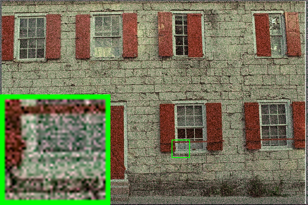
\includegraphics[width=1\textwidth]{24images/resize_br_Noisy_nSig402030_kodim01.png}}
{\footnotesize (a) Noisy kodim01: 18.44dB }
\end{minipage}
\begin{minipage}[t]{0.24\textwidth}
\centering
\raisebox{-0.15cm}{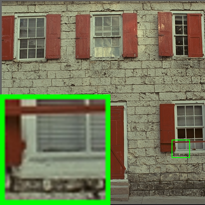
\includegraphics[width=1\textwidth]{24images/resize_br_kodim01.png}}
{\footnotesize (b) Original kodim01}
\end{minipage}
}\vspace{-2mm}
\subfigure{
\begin{minipage}[t]{0.24\textwidth}
\centering
\raisebox{-0.15cm}{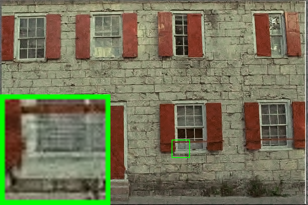
\includegraphics[width=1\textwidth]{24images/resize_br_CBM3D_nSig402030_kodim01.png}}
{\footnotesize (c) CBM3D \cite{cbm3d}: 25.24dB}
\end{minipage}
\begin{minipage}[t]{0.24\textwidth}
\centering
\raisebox{-0.15cm}{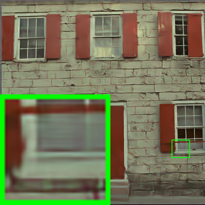
\includegraphics[width=1\textwidth]{24images/resize_br_MLP_nSig402030_kodim01.png}}
{\footnotesize (d) MLP \cite{mlp}: 25.70dB}
\end{minipage}
\begin{minipage}[t]{0.24\textwidth}
\centering
\raisebox{-0.15cm}{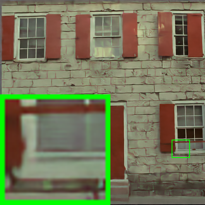
\includegraphics[width=1\textwidth]{24images/resize_br_TNRD_nSig402030_kodim01.png}}
{\footnotesize (e) TNRD \cite{chen2015learning}: 25.74dB }
\end{minipage}
\centering
\begin{minipage}[t]{0.24\textwidth}
\centering
\raisebox{-0.15cm}{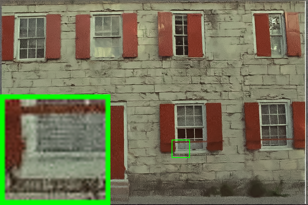
\includegraphics[width=1\textwidth]{24images/resize_br_NC_nSig402030_kodim01.png}}
{\footnotesize (f) NC \cite{noiseclinic,ncwebsite}: 24.90dB  } 
\end{minipage}
}\vspace{-2mm}
\subfigure{
\begin{minipage}[t]{0.24\textwidth}
\centering
\raisebox{-0.15cm}{\includegraphics[width=1\textwidth]{24images/resize_br_WNNMCW_nSig402030_kodim01.png}}
{\footnotesize (g) WNNM-1 \cite{wnnm}: 26.01dB  }
\end{minipage}
\begin{minipage}[t]{0.24\textwidth}
\centering
\raisebox{-0.15cm}{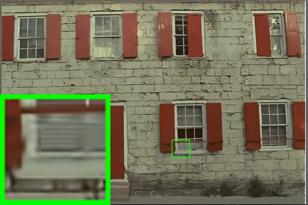
\includegraphics[width=1\textwidth]{24images/resize_br_WNNMJ_nSig402030_kodim01.png}}
{\footnotesize (h) WNNM-2: 25.95dB  }
\end{minipage}
\begin{minipage}[t]{0.24\textwidth}
\centering
\raisebox{-0.15cm}{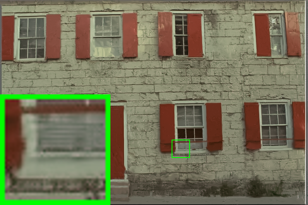
\includegraphics[width=1\textwidth]{24images/resize_br_WNNM_ADMM_nSig402030_kodim01.png}}
{\footnotesize (i) WNNM-3: 25.58dB }
\end{minipage}
\begin{minipage}[t]{0.24\textwidth}
\centering
\raisebox{-0.15cm}{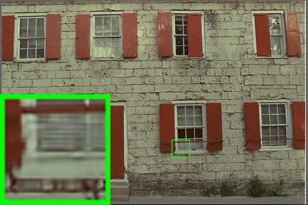
\includegraphics[width=1\textwidth]{24images/resize_br_CWNNM_ADMM_nSig402030_kodim01.png}}
{\footnotesize (j) MC-WNNM: \textbf{26.66}dB}
\end{minipage}
}
\caption{Denoised images of different methods on the image ``kodim01'' degraded by AWGN with different standard deviations of $\sigma_{r}=40, \sigma_{g}=20, \sigma_{b}=30$ on R, G, B channels, respectively. The images are better to be zoomed in on screen.}
\label{f1}
\end{figure}


%------------------------------------------------------------------------------------
\begin{figure}[!htbp]
\centering
\subfigure{
\begin{minipage}[t]{0.24\textwidth}
\centering
\raisebox{-0.15cm}{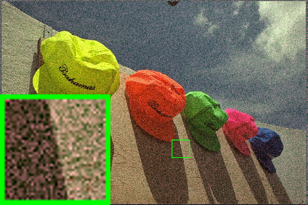
\includegraphics[width=1\textwidth]{24images/resize_br_Noisy_nSig402030_kodim03.png}}
{\footnotesize (a) Noisy kodim03: 18.56dB }
\end{minipage}
\begin{minipage}[t]{0.24\textwidth}
\centering
\raisebox{-0.15cm}{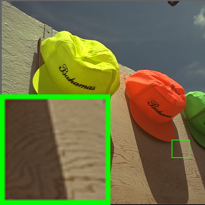
\includegraphics[width=1\textwidth]{24images/resize_br_kodim03.png}}
{\footnotesize (b) Original kodim03}
\end{minipage}
}\vspace{-2mm}
\subfigure{
\begin{minipage}[t]{0.24\textwidth}
\centering
\raisebox{-0.15cm}{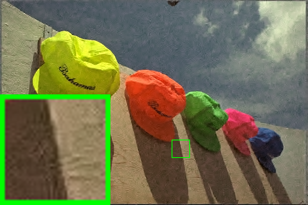
\includegraphics[width=1\textwidth]{24images/resize_br_CBM3D_nSig402030_kodim03.png}}
{\footnotesize (c) CBM3D \cite{cbm3d}: 28.81dB}
\end{minipage}
\begin{minipage}[t]{0.24\textwidth}
\centering
\raisebox{-0.15cm}{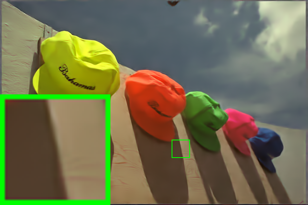
\includegraphics[width=1\textwidth]{24images/resize_br_MLP_nSig402030_kodim03.png}}
{\footnotesize (d) MLP \cite{mlp}: 31.19dB}
\end{minipage}
\begin{minipage}[t]{0.24\textwidth}
\centering
\raisebox{-0.15cm}{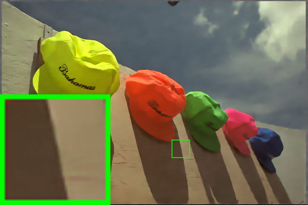
\includegraphics[width=1\textwidth]{24images/resize_br_TNRD_nSig402030_kodim03.png}}
{\footnotesize (e) TNRD \cite{chen2015learning}: 31.49dB }
\end{minipage}
\centering
\begin{minipage}[t]{0.24\textwidth}
\centering
\raisebox{-0.15cm}{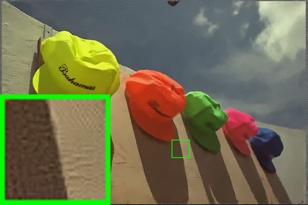
\includegraphics[width=1\textwidth]{24images/resize_br_NC_nSig402030_kodim03.png}}
{\footnotesize (f) NC \cite{noiseclinic,ncwebsite}: 28.58dB  } 
\end{minipage}
}\vspace{-2mm}
\subfigure{
\begin{minipage}[t]{0.24\textwidth}
\centering
\raisebox{-0.15cm}{\includegraphics[width=1\textwidth]{24images/resize_br_WNNMCW_nSig402030_kodim03.png}}
{\footnotesize (g) WNNM-1 \cite{wnnm}: 31.58dB  }
\end{minipage}
\begin{minipage}[t]{0.24\textwidth}
\centering
\raisebox{-0.15cm}{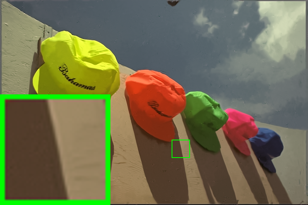
\includegraphics[width=1\textwidth]{24images/resize_br_WNNMJ_nSig402030_kodim03.png}}
{\footnotesize (h) WNNM-2: 31.61dB  }
\end{minipage}
\begin{minipage}[t]{0.24\textwidth}
\centering
\raisebox{-0.15cm}{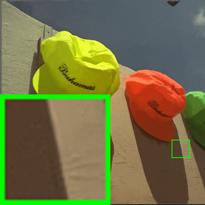
\includegraphics[width=1\textwidth]{24images/resize_br_WNNM_ADMM_nSig402030_kodim03.png}}
{\footnotesize (i) WNNM-3: 31.20dB }
\end{minipage}
\begin{minipage}[t]{0.24\textwidth}
\centering
\raisebox{-0.15cm}{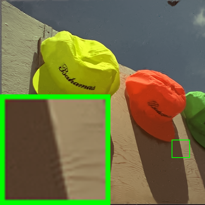
\includegraphics[width=1\textwidth]{24images/resize_br_CWNNM_ADMM_nSig402030_kodim03.png}}
{\footnotesize (j) MC-WNNM: \textbf{32.25}dB}
\end{minipage}
}
\caption{Denoised images of different methods on the image ``kodim03'' degraded by AWGN with different standard deviations of $\sigma_{r}=40, \sigma_{g}=20, \sigma_{b}=30$ on R, G, B channels, respectively. The images are better to be zoomed in on screen.}
\label{f2}
\end{figure}

%------------------------------------------------------------------------------------
\begin{figure}[!htbp]
\centering
\subfigure{
\begin{minipage}[t]{0.24\textwidth}
\centering
\raisebox{-0.15cm}{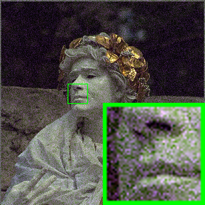
\includegraphics[width=1\textwidth]{24images/resize_br_Noisy_nSig301050_kodim17.png}}
{\footnotesize (a) Noisy kodim17: 18.33dB }
\end{minipage}
\begin{minipage}[t]{0.24\textwidth}
\centering
\raisebox{-0.15cm}{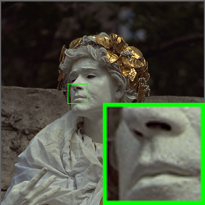
\includegraphics[width=1\textwidth]{24images/resize_br_kodim17.png}}
{\footnotesize (b) Original kodim17}
\end{minipage}
}\vspace{-2mm}
\subfigure{
\begin{minipage}[t]{0.24\textwidth}
\centering
\raisebox{-0.15cm}{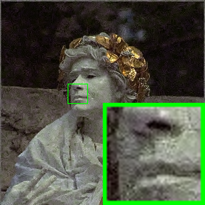
\includegraphics[width=1\textwidth]{24images/resize_br_CBM3D_nSig301050_kodim17.png}}
{\footnotesize (c) CBM3D \cite{cbm3d}: 25.12dB}
\end{minipage}
\begin{minipage}[t]{0.24\textwidth}
\centering
\raisebox{-0.15cm}{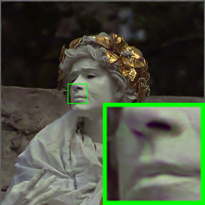
\includegraphics[width=1\textwidth]{24images/resize_br_MLP_nSig301050_kodim17.png}}
{\footnotesize (d) MLP \cite{mlp}: 30.26dB}
\end{minipage}
\begin{minipage}[t]{0.24\textwidth}
\centering
\raisebox{-0.15cm}{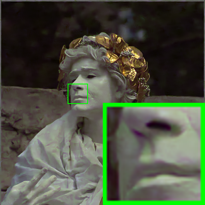
\includegraphics[width=1\textwidth]{24images/resize_br_TNRD_nSig301050_kodim17.png}}
{\footnotesize (e) TNRD \cite{chen2015learning}: 30.24dB }
\end{minipage}
\centering
\begin{minipage}[t]{0.24\textwidth}
\centering
\raisebox{-0.15cm}{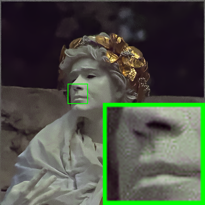
\includegraphics[width=1\textwidth]{24images/resize_br_NC_nSig301050_kodim17.png}}
{\footnotesize (f) NC \cite{noiseclinic,ncwebsite}: 27.54dB  } 
\end{minipage}
}\vspace{-2mm}
\subfigure{
\begin{minipage}[t]{0.24\textwidth}
\centering
\raisebox{-0.15cm}{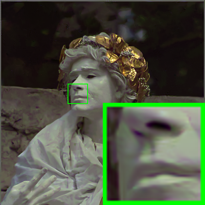
\includegraphics[width=1\textwidth]{24images/resize_br_WNNMcw_nSig301050_kodim17.png}}
{\footnotesize (g) WNNM-1 \cite{wnnm}: 30.11dB  }
\end{minipage}
\begin{minipage}[t]{0.24\textwidth}
\centering
\raisebox{-0.15cm}{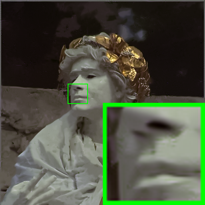
\includegraphics[width=1\textwidth]{24images/resize_br_WNNMJ_nSig301050_kodim17.png}}
{\footnotesize (h) WNNM-2: 29.35dB  }
\end{minipage}
\begin{minipage}[t]{0.24\textwidth}
\centering
\raisebox{-0.15cm}{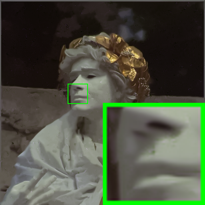
\includegraphics[width=1\textwidth]{24images/resize_br_WNNM_ADMM_nSig301050_kodim17.png}}
{\footnotesize (i) WNNM-3: 28.43dB }
\end{minipage}
\begin{minipage}[t]{0.24\textwidth}
\centering
\raisebox{-0.15cm}{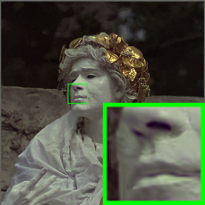
\includegraphics[width=1\textwidth]{24images/resize_br_CWNNM_ADMM_nSig301050_kodim17.png}}
{\footnotesize (j) MC-WNNM: \textbf{31.08}dB}
\end{minipage}
}
\caption{Denoised images of different methods on the image ``kodim17'' degraded by AWGN with different standard deviations of $\sigma_{r}=30, \sigma_{g}=10, \sigma_{b}=50$ on R, G, B channels, respectively. The images are better to be zoomed in on screen.}
\label{f3}
\end{figure}

%------------------------------------------------------------------------------------
\begin{figure}[!htbp]
\centering
\subfigure{
\begin{minipage}[t]{0.24\textwidth}
\centering
\raisebox{-0.15cm}{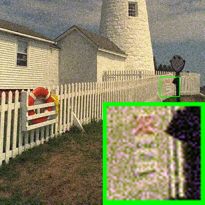
\includegraphics[width=1\textwidth]{24images/resize_br_Noisy_nSig301050_kodim19.png}}
{\footnotesize (a) Noisy kodim19: 17.92dB }
\end{minipage}
\begin{minipage}[t]{0.24\textwidth}
\centering
\raisebox{-0.15cm}{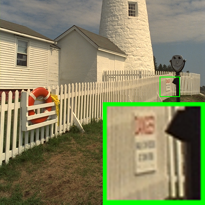
\includegraphics[width=1\textwidth]{24images/resize_br_kodim19.png}}
{\footnotesize (b) Original kodim19}
\end{minipage}
}\vspace{-2mm}
\subfigure{
\begin{minipage}[t]{0.24\textwidth}
\centering
\raisebox{-0.15cm}{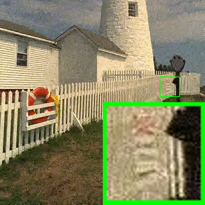
\includegraphics[width=1\textwidth]{24images/resize_br_CBM3D_nSig301050_kodim19.png}}
{\footnotesize (c) CBM3D \cite{cbm3d}: 24.63dB}
\end{minipage}
\begin{minipage}[t]{0.24\textwidth}
\centering
\raisebox{-0.15cm}{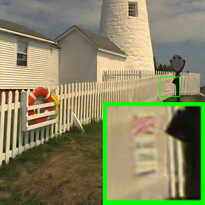
\includegraphics[width=1\textwidth]{24images/resize_br_MLP_nSig301050_kodim19.png}}
{\footnotesize (d) MLP \cite{mlp}: 29.40dB}
\end{minipage}
\begin{minipage}[t]{0.24\textwidth}
\centering
\raisebox{-0.15cm}{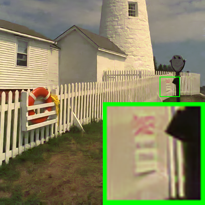
\includegraphics[width=1\textwidth]{24images/resize_br_TNRD_nSig301050_kodim19.png}}
{\footnotesize (e) TNRD \cite{chen2015learning}: 29.39dB }
\end{minipage}
\centering
\begin{minipage}[t]{0.24\textwidth}
\centering
\raisebox{-0.15cm}{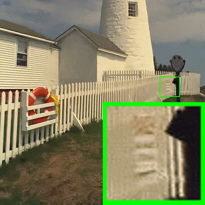
\includegraphics[width=1\textwidth]{24images/resize_br_NC_nSig301050_kodim19.png}}
{\footnotesize (f) NC \cite{noiseclinic,ncwebsite}: 27.41dB  } 
\end{minipage}
}\vspace{-2mm}
\subfigure{
\begin{minipage}[t]{0.24\textwidth}
\centering
\raisebox{-0.15cm}{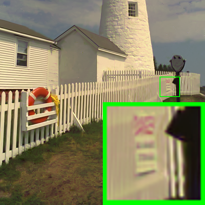
\includegraphics[width=1\textwidth]{24images/resize_br_WNNMcw_nSig301050_kodim19.png}}
{\footnotesize (g) WNNM-1 \cite{wnnm}: 29.78dB  }
\end{minipage}
\begin{minipage}[t]{0.24\textwidth}
\centering
\raisebox{-0.15cm}{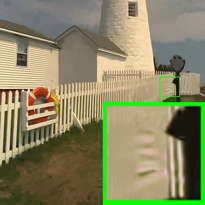
\includegraphics[width=1\textwidth]{24images/resize_br_WNNMJ_nSig301050_kodim19.png}}
{\footnotesize (h) WNNM-2: 28.87dB  }
\end{minipage}
\begin{minipage}[t]{0.24\textwidth}
\centering
\raisebox{-0.15cm}{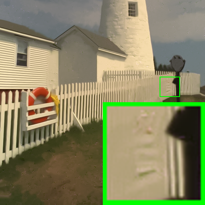
\includegraphics[width=1\textwidth]{24images/resize_br_WNNM_ADMM_nSig301050_kodim19.png}}
{\footnotesize (i) WNNM-3: 28.05dB }
\end{minipage}
\begin{minipage}[t]{0.24\textwidth}
\centering
\raisebox{-0.15cm}{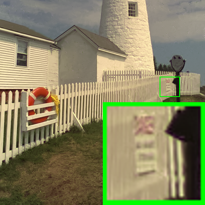
\includegraphics[width=1\textwidth]{24images/resize_br_CWNNM_ADMM_nSig301050_kodim19.png}}
{\footnotesize (j) MC-WNNM: \textbf{30.53}dB}
\end{minipage}
}
\caption{Denoised images of different methods on the image ``kodim19'' degraded by AWGN with different standard deviations of $\sigma_{r}=30, \sigma_{g}=10, \sigma_{b}=50$ on R, G, B channels, respectively. The images are better to be zoomed in on screen.}
\label{f4}
\end{figure}



%------------------------------------------------------------------------------------
\begin{figure}[!htbp]
\centering
\subfigure{
\begin{minipage}[t]{0.24\textwidth}
\centering
\raisebox{-0.15cm}{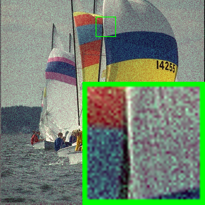
\includegraphics[width=1\textwidth]{24images/resize_br_Noisy_nSig53015_kodim09.png}}
{\footnotesize (a) Noisy kodim09: 22.36dB }
\end{minipage}
\begin{minipage}[t]{0.24\textwidth}
\centering
\raisebox{-0.15cm}{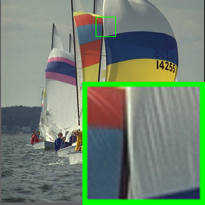
\includegraphics[width=1\textwidth]{24images/resize_br_kodim09.png}}
{\footnotesize (b) Original kodim09}
\end{minipage}
}\vspace{-2mm}
\subfigure{
\begin{minipage}[t]{0.24\textwidth}
\centering
\raisebox{-0.15cm}{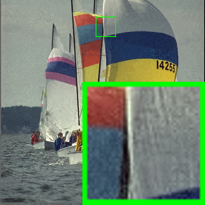
\includegraphics[width=1\textwidth]{24images/resize_br_CBM3D_nSig53015_kodim09.png}}
{\footnotesize (c) CBM3D \cite{cbm3d}: 30.07dB}
\end{minipage}
\begin{minipage}[t]{0.24\textwidth}
\centering
\raisebox{-0.15cm}{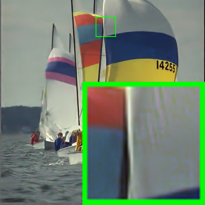
\includegraphics[width=1\textwidth]{24images/resize_br_MLP_nSig53015_kodim09.png}}
{\footnotesize (d) MLP \cite{mlp}: 31.63dB}
\end{minipage}
\begin{minipage}[t]{0.24\textwidth}
\centering
\raisebox{-0.15cm}{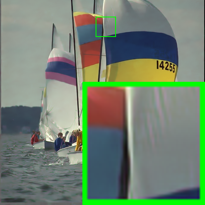
\includegraphics[width=1\textwidth]{24images/resize_br_TNRD_nSig53015_kodim09.png}}
{\footnotesize (e) TNRD \cite{chen2015learning}: 33.55dB }
\end{minipage}
\centering
\begin{minipage}[t]{0.24\textwidth}
\centering
\raisebox{-0.15cm}{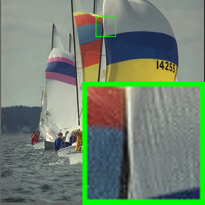
\includegraphics[width=1\textwidth]{24images/resize_br_NC_nSig53015_kodim09.png}}
{\footnotesize (f) NC \cite{noiseclinic,ncwebsite}: 31.54dB  } 
\end{minipage}
}\vspace{-2mm}
\subfigure{
\begin{minipage}[t]{0.24\textwidth}
\centering
\raisebox{-0.15cm}{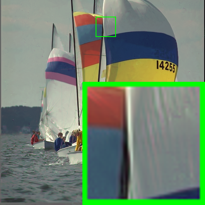
\includegraphics[width=1\textwidth]{24images/resize_br_WNNMcw_nSig53015_kodim09.png}}
{\footnotesize (g) WNNM-1 \cite{wnnm}: 33.19dB  }
\end{minipage}
\begin{minipage}[t]{0.24\textwidth}
\centering
\raisebox{-0.15cm}{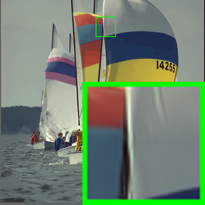
\includegraphics[width=1\textwidth]{24images/resize_br_WNNMJ_nSig53015_kodim09.png}}
{\footnotesize (h) WNNM-2: 33.20dB  }
\end{minipage}
\begin{minipage}[t]{0.24\textwidth}
\centering
\raisebox{-0.15cm}{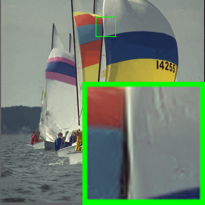
\includegraphics[width=1\textwidth]{24images/resize_br_WNNM_ADMM_nSig53015_kodim09.png}}
{\footnotesize (i) WNNM-3: 32.95dB }
\end{minipage}
\begin{minipage}[t]{0.24\textwidth}
\centering
\raisebox{-0.15cm}{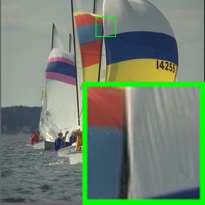
\includegraphics[width=1\textwidth]{24images/resize_br_CWNNM_ADMM_nSig53015_kodim09.png}}
{\footnotesize (j) MC-WNNM: \textbf{34.53}dB}
\end{minipage}
}
\caption{Denoised images of different methods on the image ``kodim09'' degraded by AWGN with different standard deviations of $\sigma_{r}=5, \sigma_{g}=30, \sigma_{b}=15$ on R, G, B channels, respectively. The images are better to be zoomed in on screen.}
\label{f5}
\end{figure}




%------------------------------------------------------------------------------------
\begin{figure}[!htbp]
\centering
\subfigure{
\begin{minipage}[t]{0.24\textwidth}
\centering
\raisebox{-0.15cm}{\includegraphics[width=1\textwidth]{24images/resize_br_Noisy_nSig53015_kodim15.png}}
{\footnotesize (a) Noisy kodim15: 22.23dB }
\end{minipage}
\begin{minipage}[t]{0.24\textwidth}
\centering
\raisebox{-0.15cm}{\includegraphics[width=1\textwidth]{24images/resize_br_kodim15.png}}
{\footnotesize (b) Original kodim15}
\end{minipage}
}\vspace{-2mm}
\subfigure{
\begin{minipage}[t]{0.24\textwidth}
\centering
\raisebox{-0.15cm}{\includegraphics[width=1\textwidth]{24images/resize_br_CBM3D_nSig53015_kodim15.png}}
{\footnotesize (c) CBM3D \cite{cbm3d}: 29.91dB}
\end{minipage}
\begin{minipage}[t]{0.24\textwidth}
\centering
\raisebox{-0.15cm}{\includegraphics[width=1\textwidth]{24images/resize_br_MLP_nSig53015_kodim15.png}}
{\footnotesize (d) MLP \cite{mlp}: 31.58dB}
\end{minipage}
\begin{minipage}[t]{0.24\textwidth}
\centering
\raisebox{-0.15cm}{\includegraphics[width=1\textwidth]{24images/resize_br_TNRD_nSig53015_kodim15.png}}
{\footnotesize (e) TNRD \cite{chen2015learning}: 33.13dB }
\end{minipage}
\centering
\begin{minipage}[t]{0.24\textwidth}
\centering
\raisebox{-0.15cm}{\includegraphics[width=1\textwidth]{24images/resize_br_NC_nSig53015_kodim15.png}}
{\footnotesize (f) NC \cite{noiseclinic,ncwebsite}: 31.17dB  } 
\end{minipage}
}\vspace{-2mm}
\subfigure{
\begin{minipage}[t]{0.24\textwidth}
\centering
\raisebox{-0.15cm}{\includegraphics[width=1\textwidth]{24images/resize_br_WNNMcw_nSig53015_kodim15.png}}
{\footnotesize (g) WNNM-1 \cite{wnnm}: 33.22dB  }
\end{minipage}
\begin{minipage}[t]{0.24\textwidth}
\centering
\raisebox{-0.15cm}{\includegraphics[width=1\textwidth]{24images/resize_br_WNNMJ_nSig53015_kodim15.png}}
{\footnotesize (h) WNNM-2: 32.34dB  }
\end{minipage}
\begin{minipage}[t]{0.24\textwidth}
\centering
\raisebox{-0.15cm}{\includegraphics[width=1\textwidth]{24images/resize_br_WNNM_ADMM_nSig53015_kodim15.png}}
{\footnotesize (i) WNNM-3: 32.36dB }
\end{minipage}
\begin{minipage}[t]{0.24\textwidth}
\centering
\raisebox{-0.15cm}{\includegraphics[width=1\textwidth]{24images/resize_br_CWNNM_ADMM_nSig53015_kodim15.png}}
{\footnotesize (j) MC-WNNM: \textbf{34.27}dB}
\end{minipage}
}
\caption{Denoised images of different methods on the image ``kodim15'' degraded by AWGN with different standard deviations of $\sigma_{r}=5, \sigma_{g}=30, \sigma_{b}=15$ on R, G, B channels, respectively. The images are better to be zoomed in on screen.}
\label{f6}
\end{figure}



%------------------------------------------------------------------------------------
\begin{figure}[!htbp]
\centering
\vspace{-2mm}
\subfigure{
\begin{minipage}[t]{0.3\textwidth}
\centering
\raisebox{-0.15cm}{\includegraphics[width=1\textwidth]{imagessupp/resize_br_Noisy_frog.png}}
{\footnotesize (a) Noisy \cite{ncwebsite}   }
\end{minipage}
}\vspace{-4mm}
\subfigure{
\begin{minipage}[t]{0.3\textwidth}
\centering
\raisebox{-0.15cm}{\includegraphics[width=1\textwidth]{imagessupp/resize_br_CBM3D_frog.png}}
{\footnotesize (b) CBM3D \cite{cbm3d}  }
\end{minipage}
\begin{minipage}[t]{0.3\textwidth}
\centering
\raisebox{-0.15cm}{\includegraphics[width=1\textwidth]{imagessupp/resize_br_MLP_frog.png}}
{\footnotesize (c) MLP \cite{mlp}  }
\end{minipage}
\begin{minipage}[t]{0.3\textwidth}
\centering
\raisebox{-0.15cm}{\includegraphics[width=1\textwidth]{imagessupp/resize_br_TNRD_frog.png}}
{\footnotesize (d) TNRD \cite{chen2015learning}}
\end{minipage}
}\vspace{-4mm}
\subfigure{
\begin{minipage}[t]{0.3\textwidth}
\centering
\raisebox{-0.15cm}{\includegraphics[width=1\textwidth]{imagessupp/resize_br_NI_frog.png}}
{\footnotesize (e) NI \cite{neatimage}  }
\end{minipage}
\begin{minipage}[t]{0.3\textwidth}
\centering
\raisebox{-0.15cm}{\includegraphics[width=1\textwidth]{imagessupp/resize_br_NC_frog.png}}
{\footnotesize (f) NC \cite{noiseclinic,ncwebsite}   }
\end{minipage}
\begin{minipage}[t]{0.3\textwidth}
\centering
\raisebox{-0.15cm}{\includegraphics[width=1\textwidth]{imagessupp/resize_br_WNNMcw_frog.png}}
{\footnotesize (g) WNNM-1 \cite{wnnm}   }
\end{minipage}
}\vspace{-4mm}
\subfigure{
\begin{minipage}[t]{0.3\textwidth}
\centering
\raisebox{-0.15cm}{\includegraphics[width=1\textwidth]{imagessupp/resize_br_WNNMJ_frog.png}}
{\footnotesize (h) WNNM-2   }
\end{minipage}
\begin{minipage}[t]{0.3\textwidth}
\centering
\raisebox{-0.15cm}{\includegraphics[width=1\textwidth]{imagessupp/resize_br_WNNM_ADMM_frog.png}}
{\footnotesize (i) WNNM-3   }
\end{minipage}
\begin{minipage}[t]{0.3\textwidth}
\centering
\raisebox{-0.15cm}{\includegraphics[width=1\textwidth]{imagessupp/resize_br_CWNNM_ADMM_NL_frog.png}}
{\footnotesize (j) MC-WNNM  }
\end{minipage}
}
\vspace{-1mm}
\caption{Denoised images of the real noisy image ``Frog'' \cite{ncwebsite} by different methods.\ The images are better to be zoomed in on screen.}
\label{f7}
\end{figure}


%------------------------------------------------------------------------------------
\begin{figure}[!htbp]
\centering
\vspace{-2mm}
\subfigure{
\begin{minipage}[t]{0.3\textwidth}
\centering
\raisebox{-0.15cm}{\includegraphics[width=1\textwidth]{imagessupp/resize_br_Noisy_chinesegirl.png}}
{\footnotesize (a) Noisy \cite{ncwebsite}   }
\end{minipage}
}\vspace{-4mm}
\subfigure{
\begin{minipage}[t]{0.3\textwidth}
\centering
\raisebox{-0.15cm}{\includegraphics[width=1\textwidth]{imagessupp/resize_br_CBM3D_chinesegirl.png}}
{\footnotesize (b) CBM3D \cite{cbm3d}  }
\end{minipage}
\begin{minipage}[t]{0.3\textwidth}
\centering
\raisebox{-0.15cm}{\includegraphics[width=1\textwidth]{imagessupp/resize_br_MLP_chinesegirl.png}}
{\footnotesize (c) MLP \cite{mlp}  }
\end{minipage}
\begin{minipage}[t]{0.3\textwidth}
\centering
\raisebox{-0.15cm}{\includegraphics[width=1\textwidth]{imagessupp/resize_br_TNRD_chinesegirl.png}}
{\footnotesize (d) TNRD \cite{chen2015learning}}
\end{minipage}
}\vspace{-4mm}
\subfigure{
\begin{minipage}[t]{0.3\textwidth}
\centering
\raisebox{-0.15cm}{\includegraphics[width=1\textwidth]{imagessupp/resize_br_NI_chinesegirl.png}}
{\footnotesize (e) NI \cite{neatimage}  }
\end{minipage}
\begin{minipage}[t]{0.3\textwidth}
\centering
\raisebox{-0.15cm}{\includegraphics[width=1\textwidth]{imagessupp/resize_br_NC_chinesegirl.png}}
{\footnotesize (f) NC \cite{noiseclinic,ncwebsite}   }
\end{minipage}
\begin{minipage}[t]{0.3\textwidth}
\centering
\raisebox{-0.15cm}{\includegraphics[width=1\textwidth]{imagessupp/resize_br_WNNMcw_chinesegirl.png}}
{\footnotesize (g) WNNM-1 \cite{wnnm}   }
\end{minipage}
}\vspace{-4mm}
\subfigure{
\begin{minipage}[t]{0.3\textwidth}
\centering
\raisebox{-0.15cm}{\includegraphics[width=1\textwidth]{imagessupp/resize_br_WNNMJ_chinesegirl.png}}
{\footnotesize (h) WNNM-2   }
\end{minipage}
\begin{minipage}[t]{0.3\textwidth}
\centering
\raisebox{-0.15cm}{\includegraphics[width=1\textwidth]{imagessupp/resize_br_WNNM_ADMM_chinesegirl.png}}
{\footnotesize (i) WNNM-3   }
\end{minipage}
\begin{minipage}[t]{0.3\textwidth}
\centering
\raisebox{-0.15cm}{\includegraphics[width=1\textwidth]{imagessupp/resize_br_CWNNM_ADMM_NL_chinesegirl.png}}
{\footnotesize (j) MC-WNNM  }
\end{minipage}
}
\vspace{-1mm}
\caption{Denoised images of the real noisy image ``Girl'' \cite{ncwebsite} by different methods.\ The images are better to be zoomed in on screen.}
\label{f8}
\end{figure}


%------------------------------------------------------------------------------------
\begin{figure}[!htbp]
\centering
\vspace{-2mm}
\subfigure{
\begin{minipage}[t]{0.3\textwidth}
\centering
\raisebox{-0.15cm}{\includegraphics[width=1\textwidth]{imagessupp/resize_br_Noisy_circuit.png}}
{\footnotesize (a) Noisy \cite{ncwebsite}   }
\end{minipage}
}\vspace{-4mm}
\subfigure{
\begin{minipage}[t]{0.3\textwidth}
\centering
\raisebox{-0.15cm}{\includegraphics[width=1\textwidth]{imagessupp/resize_br_CBM3D_circuit.png}}
{\footnotesize (b) CBM3D \cite{cbm3d}  }
\end{minipage}
\begin{minipage}[t]{0.3\textwidth}
\centering
\raisebox{-0.15cm}{\includegraphics[width=1\textwidth]{imagessupp/resize_br_MLP_circuit.png}}
{\footnotesize (c) MLP \cite{mlp}  }
\end{minipage}
\begin{minipage}[t]{0.3\textwidth}
\centering
\raisebox{-0.15cm}{\includegraphics[width=1\textwidth]{imagessupp/resize_br_TNRD_circuit.png}}
{\footnotesize (d) TNRD \cite{chen2015learning}}
\end{minipage}
}\vspace{-4mm}
\subfigure{
\begin{minipage}[t]{0.3\textwidth}
\centering
\raisebox{-0.15cm}{\includegraphics[width=1\textwidth]{imagessupp/resize_br_NI_circuit.png}}
{\footnotesize (e) NI \cite{neatimage}  }
\end{minipage}
\begin{minipage}[t]{0.3\textwidth}
\centering
\raisebox{-0.15cm}{\includegraphics[width=1\textwidth]{imagessupp/resize_br_NC_circuit.png}}
{\footnotesize (f) NC \cite{noiseclinic,ncwebsite}   }
\end{minipage}
\begin{minipage}[t]{0.3\textwidth}
\centering
\raisebox{-0.15cm}{\includegraphics[width=1\textwidth]{imagessupp/resize_br_WNNMcw_circuit.png}}
{\footnotesize (g) WNNM-1 \cite{wnnm}   }
\end{minipage}
}\vspace{-4mm}
\subfigure{
\begin{minipage}[t]{0.3\textwidth}
\centering
\raisebox{-0.15cm}{\includegraphics[width=1\textwidth]{imagessupp/resize_br_WNNMJ_circuit.png}}
{\footnotesize (h) WNNM-2   }
\end{minipage}
\begin{minipage}[t]{0.3\textwidth}
\centering
\raisebox{-0.15cm}{\includegraphics[width=1\textwidth]{imagessupp/resize_br_WNNM_ADMM_circuit.png}}
{\footnotesize (i) WNNM-3   }
\end{minipage}
\begin{minipage}[t]{0.3\textwidth}
\centering
\raisebox{-0.15cm}{\includegraphics[width=1\textwidth]{imagessupp/resize_br_CWNNM_ADMM_NL_circuit.png}}
{\footnotesize (j) MC-WNNM  }
\end{minipage}
}
\vspace{-1mm}
\caption{Denoised images of the real noisy image ``Circuit'' \cite{ncwebsite} by different methods.\ The images are better to be zoomed in on screen.}
\label{f9}
\end{figure}


%------------------------------------------------------------------------------------
\begin{figure}[!htbp]
\centering
\vspace{-2mm}
\subfigure{
\begin{minipage}[t]{0.3\textwidth}
\centering
\raisebox{-0.15cm}{\includegraphics[width=1\textwidth]{imagessupp/resize_br_Noisy_room.png}}
{\footnotesize (a) Noisy \cite{ncwebsite}   }
\end{minipage}
}\vspace{-4mm}
\subfigure{
\begin{minipage}[t]{0.3\textwidth}
\centering
\raisebox{-0.15cm}{\includegraphics[width=1\textwidth]{imagessupp/resize_br_CBM3D_room.png}}
{\footnotesize (b) CBM3D \cite{cbm3d}  }
\end{minipage}
\begin{minipage}[t]{0.3\textwidth}
\centering
\raisebox{-0.15cm}{\includegraphics[width=1\textwidth]{imagessupp/resize_br_MLP_room.png}}
{\footnotesize (c) MLP \cite{mlp}  }
\end{minipage}
\begin{minipage}[t]{0.3\textwidth}
\centering
\raisebox{-0.15cm}{\includegraphics[width=1\textwidth]{imagessupp/resize_br_TNRD_room.png}}
{\footnotesize (d) TNRD \cite{chen2015learning}}
\end{minipage}
}\vspace{-4mm}
\subfigure{
\begin{minipage}[t]{0.3\textwidth}
\centering
\raisebox{-0.15cm}{\includegraphics[width=1\textwidth]{imagessupp/resize_br_NI_room.png}}
{\footnotesize (e) NI \cite{neatimage}  }
\end{minipage}
\begin{minipage}[t]{0.3\textwidth}
\centering
\raisebox{-0.15cm}{\includegraphics[width=1\textwidth]{imagessupp/resize_br_NC_room.png}}
{\footnotesize (f) NC \cite{noiseclinic,ncwebsite}   }
\end{minipage}
\begin{minipage}[t]{0.3\textwidth}
\centering
\raisebox{-0.15cm}{\includegraphics[width=1\textwidth]{imagessupp/resize_br_WNNMcw_room.png}}
{\footnotesize (g) WNNM-1 \cite{wnnm}   }
\end{minipage}
}\vspace{-4mm}
\subfigure{
\begin{minipage}[t]{0.3\textwidth}
\centering
\raisebox{-0.15cm}{\includegraphics[width=1\textwidth]{imagessupp/resize_br_WNNMJ_room.png}}
{\footnotesize (h) WNNM-2   }
\end{minipage}
\begin{minipage}[t]{0.3\textwidth}
\centering
\raisebox{-0.15cm}{\includegraphics[width=1\textwidth]{imagessupp/resize_br_WNNM_ADMM_room.png}}
{\footnotesize (i) WNNM-3    }
\end{minipage}
\begin{minipage}[t]{0.3\textwidth}
\centering
\raisebox{-0.15cm}{\includegraphics[width=1\textwidth]{imagessupp/resize_br_CWNNM_ADMM_NL_room.png}}
{\footnotesize (j) MC-WNNM  }
\end{minipage}
}
\vspace{-1mm}
\caption{Denoised images of the real noisy image ``Room'' \cite{ncwebsite} by different methods.\ The images are better to be zoomed in on screen.}
\label{f10}
\end{figure}



%------------------------------------------------------------------------------------
%------------------------------------------------------------------------------------
\begin{figure}[!htbp]
\centering
\subfigure{
\begin{minipage}[t]{0.24\textwidth}
\centering
\raisebox{-0.15cm}{\includegraphics[width=1\textwidth]{comparec/resize_br_Noisy_5dmark3_iso3200_1.png}}
{\footnotesize (a) Noisy: 37.00dB }
\end{minipage}
\begin{minipage}[t]{0.24\textwidth}
\centering
\raisebox{-0.15cm}{\includegraphics[width=1\textwidth]{comparec/resize_br_5dmark3_iso3200_1.png}}
{\footnotesize (b) Mean Image \cite{crosschannel2016}}
\end{minipage}
}\vspace{-2mm}
\subfigure{
\begin{minipage}[t]{0.24\textwidth}
\centering
\raisebox{-0.15cm}{\includegraphics[width=1\textwidth]{comparec/resize_br_CBM3D_CC15_5dmark3_iso3200_1.png}}
{\footnotesize (c) CBM3D \cite{cbm3d}: 39.76dB}
\end{minipage}
\centering
\begin{minipage}[t]{0.24\textwidth}
\raisebox{-0.15cm}{\includegraphics[width=1\textwidth]{comparec/resize_br_TRD_CC15_5dmark3_iso3200_1.png}}
{\footnotesize (d)  TNRD \cite{chen2015learning}: 39.51dB}
\end{minipage}
\begin{minipage}[t]{0.24\textwidth}
\centering
\raisebox{-0.15cm}{\includegraphics[width=1\textwidth]{comparec/resize_br_NI_CC15_5dmark3_iso3200_1.png}}
{\footnotesize (e) NI \cite{neatimage}: 35.68dB }
\end{minipage}
\begin{minipage}[t]{0.24\textwidth}
\centering
\raisebox{-0.15cm}{\includegraphics[width=1\textwidth]{comparec/resize_br_NC_CC15_5dmark3_iso3200_1.png}}
{\footnotesize (f) NC \cite{noiseclinic,ncwebsite}: 36.20dB  } 
\end{minipage}
}\vspace{-2mm}
\subfigure{
\begin{minipage}[t]{0.24\textwidth}
\centering
\raisebox{-0.15cm}{\includegraphics[width=1\textwidth]{comparec/resize_br_CC_CC15_5dmark3_iso3200_1.png}}
{\footnotesize (g) CC \cite{crosschannel2016}: 38.37dB  }
\end{minipage}
\begin{minipage}[t]{0.24\textwidth}
\centering
\raisebox{-0.15cm}{\includegraphics[width=1\textwidth]{comparec/resize_br_WNNMJ_CC15_5dmark3_iso3200_1.png}}
{\footnotesize (h) WNNM-2: 39.74dB  }
\end{minipage}
\begin{minipage}[t]{0.24\textwidth}
\centering
\raisebox{-0.15cm}{\includegraphics[width=1\textwidth]{comparec/resize_br_WNNM_ADMM_NL_CC15_5dmark3_iso3200_1.png}}
{\footnotesize (i) WNNM-3: 39.98dB }
\end{minipage}
\begin{minipage}[t]{0.24\textwidth}
\centering
\raisebox{-0.15cm}{\includegraphics[width=1\textwidth]{comparec/resize_br_CWNNM_ADMM_NL_CC15_5dmark3_iso3200_1.png}}
{\footnotesize (j) MC-WNNM: \textbf{41.13}dB}
\end{minipage}
}
\caption{Denoised images of a region cropped from the real noisy image ``Canon 5D Mark 3 ISO=3200 1" \cite{crosschannel2016} by different methods. The images are better to be zoomed in on screen.}
\label{f11}
\end{figure}

\begin{figure}[!htbp]
\centering
\subfigure{
\begin{minipage}[t]{0.24\textwidth}
\centering
\raisebox{-0.15cm}{\includegraphics[width=1\textwidth]{imagessupp/resize_br_Noisy_d600_iso3200_2.png}}
{\footnotesize (a) Noisy  \cite{crosschannel2016}: 33.77dB }
\end{minipage}
\begin{minipage}[t]{0.24\textwidth}
\centering
\raisebox{-0.15cm}{\includegraphics[width=1\textwidth]{imagessupp/resize_br_d600_iso3200_2.png}}
{\footnotesize (b) Mean Image \cite{crosschannel2016}}
\end{minipage}
}\vspace{-2mm}
\subfigure{
\begin{minipage}[t]{0.24\textwidth}
\centering
\raisebox{-0.15cm}{\includegraphics[width=1\textwidth]{imagessupp/resize_br_CBM3D_CC15_d600_iso3200_2.png}}
{\footnotesize (c) CBM3D \cite{bm3d,cbm3d}: 35.07dB}
\end{minipage}
\centering
\begin{minipage}[t]{0.24\textwidth}
\raisebox{-0.15cm}{\includegraphics[width=1\textwidth]{imagessupp/resize_br_TRD_CC15_d600_iso3200_2.png}}
{\footnotesize (d) TNRD \cite{chen2015learning}: 36.37dB  } 
\end{minipage}
\begin{minipage}[t]{0.24\textwidth}
\centering
\raisebox{-0.15cm}{\includegraphics[width=1\textwidth]{imagessupp/resize_br_NI_CC15_d600_iso3200_2.png}}
{\footnotesize (e) NI \cite{neatimage}: 35.16dB  }
\end{minipage}
\begin{minipage}[t]{0.24\textwidth}
\centering
\raisebox{-0.15cm}{\includegraphics[width=1\textwidth]{imagessupp/resize_br_NC_CC15_d600_iso3200_2.png}}
{\footnotesize (f) NC \cite{ncwebsite,noiseclinic}: 35.34dB  }
\end{minipage}
}\vspace{-2mm}
\subfigure{
\begin{minipage}[t]{0.24\textwidth}
\centering
\raisebox{-0.15cm}{\includegraphics[width=1\textwidth]{imagessupp/resize_br_CC_d600_iso3200_2.png}}
{\footnotesize (g) CC \cite{crosschannel2016}: 35.95dB }
\end{minipage}
\begin{minipage}[t]{0.24\textwidth}
\centering
\raisebox{-0.15cm}{\includegraphics[width=1\textwidth]{imagessupp/resize_br_WNNMJ_CC15_d600_iso3200_2.png}}
{\footnotesize (h) WNNM-2: 36.42dB}
\end{minipage}
\begin{minipage}[t]{0.24\textwidth}
\centering
\raisebox{-0.15cm}{\includegraphics[width=1\textwidth]{imagessupp/resize_br_WNNM_ADMM_NL_CC15_d600_iso3200_2.png}}
{\footnotesize (i) WNNM-3: 36.84dB}
\end{minipage}
\begin{minipage}[t]{0.24\textwidth}
\centering
\raisebox{-0.15cm}{\includegraphics[width=1\textwidth]{imagessupp/resize_br_CWNNM_ADMM_NL_CC15_d600_iso3200_2.png}}
{\footnotesize (j) MC-WNNM: \textbf{37.02}dB}
\end{minipage}
}
\caption{Denoised images of a region cropped from the real noisy image ``Nikon D600 ISO=3200 2" \cite{crosschannel2016} by different methods. The images are better to be zoomed in on screen.}
\label{f12}
\end{figure}




%------------------------------------------------------------------------------------
\begin{figure}[!htbp]
\centering
\subfigure{
\begin{minipage}[t]{0.24\textwidth}
\centering
\raisebox{-0.15cm}{\includegraphics[width=1\textwidth]{imagessupp/resize_br_Noisy_d800_iso1600_2.png}}
{\footnotesize (a) Noisy  \cite{crosschannel2016}: 35.71dB }
\end{minipage}
\begin{minipage}[t]{0.24\textwidth}
\centering
\raisebox{-0.15cm}{\includegraphics[width=1\textwidth]{imagessupp/resize_br_d800_iso1600_2.png}}
{\footnotesize (b) Mean Image \cite{crosschannel2016}}
\end{minipage}
}\vspace{-2mm}
\subfigure{
\begin{minipage}[t]{0.24\textwidth}
\centering
\raisebox{-0.15cm}{\includegraphics[width=1\textwidth]{imagessupp/resize_br_CBM3D_CC15_d800_iso1600_2.png}}
{\footnotesize (c) CBM3D \cite{bm3d,cbm3d}: 37.76dB}
\end{minipage}
\centering
\begin{minipage}[t]{0.24\textwidth}
\raisebox{-0.15cm}{\includegraphics[width=1\textwidth]{imagessupp/resize_br_TRD_CC15_d800_iso1600_2.png}}
{\footnotesize (d) TNRD \cite{chen2015learning}: 40.52dB  } 
\end{minipage}
\begin{minipage}[t]{0.24\textwidth}
\centering
\raisebox{-0.15cm}{\includegraphics[width=1\textwidth]{imagessupp/resize_br_NI_CC15_d800_iso1600_2.png}}
{\footnotesize (e) NI \cite{neatimage}: 38.42dB  }
\end{minipage}
\begin{minipage}[t]{0.24\textwidth}
\centering
\raisebox{-0.15cm}{\includegraphics[width=1\textwidth]{imagessupp/resize_br_NC_CC15_d800_iso1600_2.png}}
{\footnotesize (f) NC \cite{ncwebsite,noiseclinic}: 38.65dB  }
\end{minipage}
}\vspace{-2mm}
\subfigure{
\begin{minipage}[t]{0.24\textwidth}
\centering
\raisebox{-0.15cm}{\includegraphics[width=1\textwidth]{imagessupp/resize_br_CC_d800_iso1600_2.png}}
{\footnotesize (g) CC \cite{crosschannel2016}: 40.36dB }
\end{minipage}
\begin{minipage}[t]{0.24\textwidth}
\centering
\raisebox{-0.15cm}{\includegraphics[width=1\textwidth]{imagessupp/resize_br_WNNMJ_CC15_d800_iso1600_2.png}}
{\footnotesize (h) WNNM-2: 41.24dB}
\end{minipage}
\begin{minipage}[t]{0.24\textwidth}
\centering
\raisebox{-0.15cm}{\includegraphics[width=1\textwidth]{imagessupp/resize_br_WNNM_ADMM_NL_CC15_d800_iso1600_2.png}}
{\footnotesize (i) WNNM-3: 40.81dB}
\end{minipage}
\begin{minipage}[t]{0.24\textwidth}
\centering
\raisebox{-0.15cm}{\includegraphics[width=1\textwidth]{imagessupp/resize_br_CWNNM_ADMM_NL_CC15_d800_iso1600_2.png}}
{\footnotesize (j) MC-WNNM: \textbf{41.43}dB}
\end{minipage}
}
\caption{Denoised images of a region cropped from the real noisy image ``Nikon D800 ISO=1600 2" \cite{crosschannel2016} by different methods. The images are better to be zoomed in on screen.}
\label{f13}
\end{figure}


%------------------------------------------------------------------------------------
\begin{figure}[!htbp]
\centering
\subfigure{
\begin{minipage}[t]{0.24\textwidth}
\centering
\raisebox{-0.15cm}{\includegraphics[width=1\textwidth]{imagessupp/resize_br_Noisy_d800_iso3200_2.png}}
{\footnotesize (a) Noisy  \cite{crosschannel2016}: 32.89dB }
\end{minipage}
\begin{minipage}[t]{0.24\textwidth}
\centering
\raisebox{-0.15cm}{\includegraphics[width=1\textwidth]{imagessupp/resize_br_d800_iso3200_2.png}}
{\footnotesize (b) Mean Image \cite{crosschannel2016}}
\end{minipage}
}\vspace{-2mm}
\subfigure{
\begin{minipage}[t]{0.24\textwidth}
\centering
\raisebox{-0.15cm}{\includegraphics[width=1\textwidth]{imagessupp/resize_br_CBM3D_CC15_d800_iso3200_2.png}}
{\footnotesize (c) CBM3D \cite{bm3d,cbm3d}: 34.07dB}
\end{minipage}
\centering
\begin{minipage}[t]{0.24\textwidth}
\raisebox{-0.15cm}{\includegraphics[width=1\textwidth]{imagessupp/resize_br_TRD_CC15_d800_iso3200_2.png}}
{\footnotesize (d) TNRD \cite{chen2015learning}: 35.90dB  } 
\end{minipage}
\begin{minipage}[t]{0.24\textwidth}
\centering
\raisebox{-0.15cm}{\includegraphics[width=1\textwidth]{imagessupp/resize_br_NI_CC15_d800_iso3200_2.png}}
{\footnotesize (e) NI \cite{neatimage}: 35.53dB  }
\end{minipage}
\begin{minipage}[t]{0.24\textwidth}
\centering
\raisebox{-0.15cm}{\includegraphics[width=1\textwidth]{imagessupp/resize_br_NC_CC15_d800_iso3200_2.png}}
{\footnotesize (f) NC \cite{ncwebsite,noiseclinic}: 35.76dB  }
\end{minipage}
}\vspace{-2mm}
\subfigure{
\begin{minipage}[t]{0.24\textwidth}
\centering
\raisebox{-0.15cm}{\includegraphics[width=1\textwidth]{imagessupp/resize_br_CC_d800_iso3200_2.png}}
{\footnotesize (g) CC \cite{crosschannel2016}: 36.75dB }
\end{minipage}
\begin{minipage}[t]{0.24\textwidth}
\centering
\raisebox{-0.15cm}{\includegraphics[width=1\textwidth]{imagessupp/resize_br_WNNMJ_CC15_d800_iso3200_2.png}}
{\footnotesize (h) WNNM-2: 37.32dB}
\end{minipage}
\begin{minipage}[t]{0.24\textwidth}
\centering
\raisebox{-0.15cm}{\includegraphics[width=1\textwidth]{imagessupp/resize_br_WNNM_ADMM_NL_CC15_d800_iso3200_2.png}}
{\footnotesize (i) WNNM-3: 37.30dB}
\end{minipage}
\begin{minipage}[t]{0.24\textwidth}
\centering
\raisebox{-0.15cm}{\includegraphics[width=1\textwidth]{imagessupp/resize_br_CWNNM_ADMM_NL_CC15_d800_iso3200_2.png}}
{\footnotesize (j) MC-WNNM: \textbf{37.41}dB}
\end{minipage}
}
\caption{Denoised images of a region cropped from the real noisy image ``Nikon D800 ISO=3200 2" \cite{crosschannel2016} by different methods. The images are better to be zoomed in on screen.}
\label{f14}
\end{figure}


\clearpage
{
\huge
%\small
\bibliographystyle{unsrt}
\bibliography{egbib}
}


\end{document}
